\documentclass[11pt]{article}
\usepackage[margin=1in]{geometry}
\usepackage[T1]{fontenc}
\usepackage{lmodern,amsmath,amssymb,booktabs,graphicx,xcolor,hyperref}
\usepackage[numbers,sort&compress]{natbib}
\usepackage{tikz,needspace,placeins}
\usetikzlibrary{arrows.meta,positioning}
\hypersetup{colorlinks=true,linkcolor=blue,citecolor=blue,urlcolor=blue}
\setlength{\emergencystretch}{2em}
\definecolor{paperteal}{HTML}{007F86}
\definecolor{paperpale}{HTML}{EDF4F3}
\renewcommand{\topfraction}{0.9}
\renewcommand{\bottomfraction}{0.85}
\renewcommand{\textfraction}{0.08}
\renewcommand{\floatpagefraction}{0.8}
\newcommand{\kj}{\ensuremath{\mathrm{kJ\,mol^{-1}}}}
\newcommand{\EmptyAllSameChange}{-1.03}
\newcommand{\EmptyAllSameUnique}{20}
\newcommand{\EmptyAlternatingChange}{-1.23}
\newcommand{\EmptyAlternatingUnique}{19}

\newcommand{\TempoReduction}{1.477}
\newcommand{\TempoOxidation}{1.639}
\newcommand{\TempoAsymmetryPercent}{10.4}
\newcommand{\TempoReductionGeometry}{0.396}
\newcommand{\TempoReductionSlow}{1.081}
\newcommand{\TempoOxidationGeometry}{0.553}
\newcommand{\TempoOxidationSlow}{1.086}

\newcommand{\MolecularFirstReduction}{-0.608}
\newcommand{\MolecularSecondReduction}{-1.208}
\newcommand{\MolecularSpacing}{0.600}
\newcommand{\MolecularDisproportionation}{57.91}

\newcommand{\ViologenGraftDG}{-11.49}
\newcommand{\ViologenGraftRotorLow}{-13.30}
\newcommand{\ViologenGraftRotorHigh}{-11.49}
\newcommand{\ViologenGraftSeedSpan}{1.50}

\newcommand{\IonicAdjacentG}{-3.94}
\newcommand{\IonicAdjacentE}{-3.46}
\newcommand{\IonicAdjacentGLow}{-5.85}
\newcommand{\IonicAdjacentGHigh}{-3.94}
\newcommand{\IonicLargeMinimum}{6.96}
\newcommand{\IonicSpacerG}{22.58}
\newcommand{\IonicSpacerE}{18.68}
\newcommand{\IonicSpacerGLow}{19.75}
\newcommand{\IonicSpacerGHigh}{22.58}
\newcommand{\IonicAlternatingSpacerG}{-5.30}
\newcommand{\IonicAlternatingSpacerGLow}{-5.79}
\newcommand{\IonicAlternatingSpacerGHigh}{-4.28}
\newcommand{\IonicAlternatingAdjacentG}{8.28}
\newcommand{\IonicAlternatingAdjacentE}{1.20}
\newcommand{\IonicAlternatingAdjacentGLow}{8.28}
\newcommand{\IonicAlternatingAdjacentGHigh}{8.37}
\newcommand{\IonicAlternatingAdjacentMinimum}{9.23}

\title{From Molecular Redox Screening to Polymer Grafts: Benchmarking and Matched Thermodynamic Comparisons}
\author{Working draft: authorship and affiliations to be confirmed}
\date{JCIM Article draft; evidence updated: 3 November 2026}
\newcommand{\MotifAdjacentE}{9.029}
\newcommand{\MotifMinimumE}{7.618}
\newcommand{\MotifMaximumE}{9.631}
\newcommand{\MotifCapSpan}{0.003}

\newcommand{\ChlorideAssocMin}{5.33}
\newcommand{\ChlorideAssocMax}{22.36}
\newcommand{\ChlorideCorrection}{-7.93}
\newcommand{\ChlorideNZeroMinus}{15.61}
\newcommand{\ChlorideNZeroPlus}{15.42}
\newcommand{\ChlorideNOneAbove}{22.36}
\newcommand{\ChlorideNOneBelow}{22.11}
\newcommand{\ChlorideNZeroBelow}{6.23}
\newcommand{\ChlorideNZeroOuter}{5.33}
\newcommand{\ChlorideNZeroOuterPlus}{5.93}
\newcommand{\ChlorideOutcomeCount}{7}
\newcommand{\ChlorideDuplicateCount}{5}

\newcommand{\UnifiedRegistryCount}{912}
\newcommand{\NewDirectPTZDesigns}{8}
\newcommand{\ReviewedRouteCount}{3}

\newcommand{\SamplingTwentyFiveAbs}{2.55}
\newcommand{\SamplingFiftyAbs}{2.40}
\newcommand{\SamplingHundredAbs}{2.54}
\newcommand{\SamplingTolerance}{2.00}
\newcommand{\SamplingMinimumEDrop}{3.88}

\newcommand{\PTZPrimaryV}{0.626}
\newcommand{\PTZLowV}{0.616}
\newcommand{\PTZHighV}{0.626}
\newcommand{\PTZBranchMicroV}{0.08}

\begin{document}
\maketitle

\begin{abstract}
We assess redox groups for attachment to preformed polymers using a 39-endpoint acetonitrile benchmark, an experimentally supported viologen attachment class, and TEMPO and diimide controls. The unfitted redox protocol gives a mean absolute error of 0.247 V; all nine paired redox-step spacings are overestimated, showing that a ferrocene reference shift cannot remove this error. Matched oligomer cycles distinguish the polymer contribution to attachment from neighboring-graft nonadditivity, and four illustrative ionic viologen frames show favorable whole-chain electronic nonadditivity coexisting with repulsive capped motif pairs. These comparisons connect molecular electrochemistry, defined attachment reactions and local polymer environments; their predictive scope remains limited by molecular redox error, salt speciation and incomplete occupied-polymer sampling.
\end{abstract}
\noindent\textbf{Keywords:} computational electrochemistry; redox-active polymers; polymer grafting; density functional theory; thermodynamic cycles; conformer sampling.

\section{Introduction}
Nonaqueous flow batteries can store charge in redox groups attached to insoluble polymer beads while soluble mediators exchange charge with those groups. This architecture separates the circulating electrolyte from the charge-storage material, making the electrochemistry of the pendant group central to the design.\cite{kim2022} Related polymer and colloidal systems illustrate the broader use of macromolecular supports to retain redox-active material.\cite{janoschka2015,montoto2016} Post-functionalization of a preformed support allows the polymer and redox group to be prepared separately; attachment to chloromethylated polystyrene has been demonstrated for viologen, TEMPO and phenothiazine groups.\cite{kim2022,sommerlade2002tempo,wright1989supported,ohbiying2025upcycling}

A molecular screening result addresses only part of this choice. The installed group has a specific attachment bond and linker. Its preparation requires a suitable precursor and reaction conditions, and its local environment depends on graft occupancy and polymer conformation. Molecular potential, installation free energy and neighboring-group response therefore answer different questions. For a redox-matched battery, the potential of the installed group must also be considered in relation to its soluble mediator, while useful capacity depends on the amount of polymer and the fraction of accessible redox sites.\cite{kim2022}

High-throughput screening and redox databases provide molecular structures and electrochemical descriptors across broad chemical spaces.\cite{er2015,d3tales2023,reddb2022} Multistep screening has also been developed for radical-polymer anodes and flow-battery anolytes.\cite{achazi2024screening} Computational electrochemistry establishes the roles of reference choice, solvation and charge-state treatment,\cite{marenich2014,fc2010,elhajj2024} while studies of diimide association and charge transport in polymers motivate explicit treatment of neighboring groups and backbone structure.\cite{wiberg2021,hopping2013,mohanty2026backbone} Together, these approaches raise a question: which molecular conclusions remain valid for an installed group and its polymer environment?

Here we address that question through a benchmark and matched thermodynamic comparisons. First, we examine the accuracy and redox-step dependence of an unfitted molecular protocol. We then follow an exact viologen graft from a source-supported attachment class through its molecular states, local quaternization reaction and finite oligomer models. Balanced differences distinguish the polymer contribution to first attachment from the effect of an occupied neighboring site. Finally, frozen motif calculations test whether whole-chain nonadditivity can be interpreted as direct motif attraction. TEMPO, pyromellitic diimide (PMDI) and phthalimide supply focused supporting comparisons. These quantitative examples provide a reproducible way to formulate and test the links between molecular, reaction and polymer calculations. They do not constitute a completed ranking of polymer materials.

\section{Computational Methods}
\subsection{Structures, reaction models and calculation levels}
The synthesis modeled here is post-functionalization of a polymer bearing benzyl chloride handles. A 4-methylbenzyl chloride site and its substituted product define the local graft model. Five-repeat open oligomers contain three reactive sites and two unfunctionalized styrene padding units; an unoccupied reactive site retains benzyl chloride. We check precursor/product graphs, attachment bonds and connectivity in the saved coordinates explicitly. Free parents, capped grafts and oligomers are treated as distinct structures. The design registry and route evidence, including the distinction between an exact-support demonstration and a molecular analogue, are provided in the Supporting Information (SI).

Molecular geometries and solution Hessians use r$^2$SCAN-D4/SMD acetonitrile (MeCN), with def2-SVP for neutral/cationic species and def2-SVPD for anions.\cite{r2scan2020,d42019,smd2009,def22005,diffuse2010} Molecular single-point electronic energies use $\omega$B97M-V/def2-TZVPD uniformly for every target charge state and both ferrocene (Fc) states.\cite{wb97mv2016} Calculations use PySCF 2.14.0, GPU4PySCF 1.8.1 and geomeTRIC, with density fitting of Coulomb and exact-exchange contributions.\cite{pyscf2020,gpu4pyscf2024,geometric2016} Supporting electrolyte ions are absent except in explicitly identified contact models.

At 298.15 K, the molecular composite free energy is
\begin{equation}
G=E_{\mathrm{SMD}}^{\omega\mathrm{B97M-V}}+G_{\mathrm{nuclear}}^{\mathrm{qRRHO}}-RT\ln(2S+1).
\label{eq:g}
\end{equation}
The quasi-rigid-rotor/harmonic-oscillator (qRRHO) nuclear partition uses projected internal modes from the solution DFT Hessian. The xTB 6.7.1 thermodynamic integrator evaluates the partition using unscaled frequencies and a geometry-specific symmetry number.\cite{grimme2012,xtbprogram2021} The Hessian is therefore calculated by DFT, not xTB. The primary rotor cutoff is 50 cm$^{-1}$; 25 and 100 cm$^{-1}$ test sensitivity. The spin term assumes an unsplit ground multiplet.

Each reported minimum must have a maximum Cartesian gradient component no greater than $4.5\times10^{-4}$ hartree bohr$^{-1}$, Hessian asymmetry no greater than $10^{-6}$ in atomic units, a lowest projected internal frequency of at least $-5$ cm$^{-1}$ and spin contamination no greater than 0.1. Frequencies between $-5$ and 0 cm$^{-1}$ enter the partition by absolute value. At least two complete Hessian columns are checked against displaced gradients at 0.0005 and 0.001 bohr with a 1\% relative-norm tolerance. We also verify that the electronic energy belongs to the accepted geometry, that the data are finite and that the calculation includes the full grid response. The SI gives derivative-selection, implementation-repeat and independent reconstruction details. These checks validate the local numerical calculations. Experimental accuracy and conformer sampling are assessed separately.

The ionic viologen oligomer cycles use r$^2$SCAN-D4/def2-SVP electronic energies and Hessians in a separate smooth-surface MeCN model. The corrected occupied-phthalimide sampling control instead combines $\omega$B97M-V/def2-TZVPD electronic energies with r$^2$SCAN-D4/def2-SVP Hessians in the declared smooth-surface model. Each comparison combines components from the same model. These control results are kept separate from the primary composite molecular reaction energies. Table~\ref{tab:levels} summarizes the calculation levels.
\begin{table}[htbp]\centering\small
\caption{Calculation levels and quantities used in the comparisons. The SI specifies the separate smooth-surface implementation and the scope of its derivative checks.}
\label{tab:levels}
\begin{tabular}{p{.25\linewidth}p{.36\linewidth}p{.29\linewidth}}\toprule
Comparison & Electronic energy & Nuclear treatment / scope\\\midrule
Parent benchmark, capped grafts and local reactions & $\omega$B97M-V/def2-TZVPD/SMD & Geometry-level DFT qRRHO; Eq.~\ref{eq:g}\\
Primary PMDI and phthalimide oligomer controls & Same composite protocol & One or two minima per graph\\
Ionic viologen oligomers & r$^2$SCAN-D4/def2-SVP, smooth-surface MeCN & Matched graph-specific qRRHO; one minimum per graph\\
Corrected occupied-phthalimide sampling & $\omega$B97M-V/def2-TZVPD, smooth-surface MeCN & r$^2$SCAN-D4/def2-SVP Hessians and projected qRRHO; nested sampling diagnostic\\
Frozen viologen motif pairs & Same electronic model as ionic parent frames & Electronic differences only; fixed motif coordinates\\\bottomrule
\end{tabular}\end{table}

\subsection{Molecular redox benchmark}
For a one-electron couple $\mathrm{O+e^-\rightarrow R}$, the potential relative to the computed Fc/Fc$^+$ reference is
\begin{equation}
E_{\mathrm{O/R}}^{\mathrm{vs\ Fc}}=
\frac{G_{\mathrm O}-G_{\mathrm R}-[G_{\mathrm{Fc^+}}-G_{\mathrm{Fc}}]}{F}.
\label{eq:redox}
\end{equation}
All four states use matched electronic and thermal conventions. Equation~\ref{eq:redox} uses molar energies; a one-electron energy difference in eV per molecule gives the voltage directly.

The fixed retrospective panel contains 39 MeCN endpoints from 30 molecules and seven studies: 22 quinone, nine aromatic-imide, five phenothiazine, two viologen and one nitroxide endpoints. Each experimental potential is recorded with its source-reported reference calibration and measurement conditions. No endpoint is removed and no offset is fitted in the primary analysis. Molecule- and study-cluster percentile bootstrap intervals use 2,000 replicates and seed 20261021. Grouped held-out offset analyses are post hoc diagnostics; each training fold excludes every endpoint of the held-out molecule or study. They are not prospective external validation. Source locations, state assignments and individual errors are supplied in the SI and accompanying benchmark data.

\subsection{Local attachment and balanced polymer comparisons}
Viologen installation is modeled as quaternization of a mono-N-methyl bipyridinium precursor with the local RCl site:
\begin{equation}
\mathrm{V_{prec}^++RCl\rightarrow RV^{2+}+Cl^-}.
\label{eq:quaternization}
\end{equation}
The reaction conserves atoms and charge and has no HCl or base-capture term. Three fixed precursor starts are checked; the lowest precursor $G$ at the primary cutoff is used. The separated-ion convention treats chloride and the dicationic graft as distinct solutes. Explicit graft/chloride contacts are tested separately using
\begin{equation}
\Delta G_{\mathrm{assoc}}=G(\mathrm{RVCl^+})-G(\mathrm{RV^{2+}})-G(\mathrm{Cl^-}).
\end{equation}
The contact is a $+1$ singlet, chemically distinct from the isolated $+1$ doublet redox state. Duplicate structures are identified by symmetry-aware heavy-atom alignment using proper rotations and an electronic-energy tolerance. The number of starts does not define populations.

The nuclear translation convention is 1 atm. Conversion to a 1 M solute standard state adds $\Delta nRT\ln(RTc^\circ/p^\circ)$. It cancels in separated-ion quaternization and contributes approximately $-7.93$ \kj\ to a two-solute-to-one-solute contact association at 298.15 K. The SI defines the separate N--H/O--H substitution cycles and base-capture controls used for the supporting neutral grafts. Those reaction definitions are not transferred to viologen quaternization.

For an empty oligomer $P_0$, a singly grafted oligomer $P_i$, local site RCl and capped graft RM, the polymer-minus-local first-attachment difference is
\begin{equation}
\delta G_{i,\mathrm{poly-local}}=G(P_i)+G(\mathrm{RCl})-G(P_0)-G(\mathrm{RM}).
\label{eq:polylocal}
\end{equation}
The neighboring-graft response uses the empty, singly occupied and doubly occupied graphs:
\begin{equation}
\Delta\Delta G_{ij}=G(P_{ij})+G(P_0)-G(P_i)-G(P_j).
\label{eq:nonadditivity}
\end{equation}
Common precursor, base and byproduct terms cancel in these balanced differences. The first difference measures the polymer contribution relative to the capped reaction. The second measures how occupation of $i$ changes attachment at $j$. Both include chain relaxation and solvent response. Neither is an isolated pair-binding free energy.

\begin{figure}[htbp]\centering
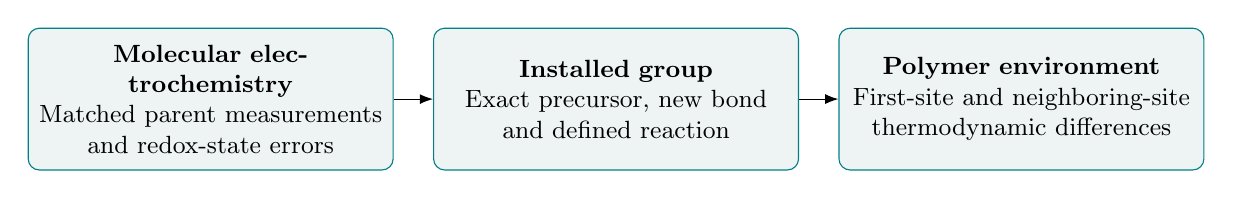
\begin{tikzpicture}[node distance=5mm,every node/.style={draw,rounded corners,align=center,font=\small,text width=4.4cm,minimum height=18mm,draw=paperteal,fill=paperpale},>=Latex]
\node (parent) {\textbf{Molecular electrochemistry}\\Matched parent measurements\\and redox-state errors};
\node[right=of parent] (graft) {\textbf{Installed group}\\Exact precursor, new bond\\and defined reaction};
\node[right=of graft] (polymer) {\textbf{Polymer environment}\\First-site and neighboring-site\\thermodynamic differences};
\draw[->] (parent)--(graft);\draw[->] (graft)--(polymer);
\end{tikzpicture}
\caption{The three comparisons addressed in the study. Measured soluble parents test the molecular protocol. A capped graft specifies the installed chemical group and its local reaction. Balanced oligomer cycles test additional environmental responses. Each comparison retains its own structure, method and reference; arrows indicate the assessment sequence.}
\label{fig:workflow}\end{figure}

\subsection{Sampling and local interaction controls}
Graph-specific finite conformer sets use
\begin{equation}
G_{\mathrm{set}}=-RT\ln\sum_k\exp[-G_k/(RT)].
\end{equation}
Duplicate structures are identified before summation. The PMDI and ionic viologen cycles use one retained minimum per graph; the original phthalimide control uses two. Expanded occupied-phthalimide sampling supplies a separate ten-to-twenty-start diagnostic under the smooth-surface model. It cannot establish convergence for a different graph or replace a primary-model component.

Frozen motif interactions are defined as $\Delta E_{\mathrm{motif}}=E_{AB}-E_A-E_B$ at unchanged parent-relative motif coordinates, using the same electronic and solvent model as the parent frame. For viologen, the benzyl carbon is retained and its aryl bond is replaced by C--H, giving methyl-capped $+2$ singlet motifs and a $+4$ singlet pair. Four frames and three C--H lengths (1.07, 1.09 and 1.11 \AA) give twelve fragment triplets. These electronic interactions include capping and continuum response but no counterpoise correction or thermal association term. The SI reports the fragment construction and the separate TEMPO directional-relaxation calculation.\cite{you2015nonequilibrium}

\section{Results and Discussion}
\subsection{Redox-step errors cannot be removed by a common reference shift}
The unfitted protocol gives MAE 0.247 V, RMSE 0.279 V and bias $+0.190$ V (Figure~\ref{fig:benchmark}). Molecule-cluster 95\% intervals are [0.213,0.286], [0.245,0.313] and [0.128,0.257] V, respectively. The panel covers several relevant families but is dominated by quinones; the five phenothiazine endpoints and single TEMPO endpoint do not establish broad family accuracy. The two viologen endpoints belong to one molecule, and naphthalene diimide (NDI) is absent.

\begin{figure}[htbp]\centering
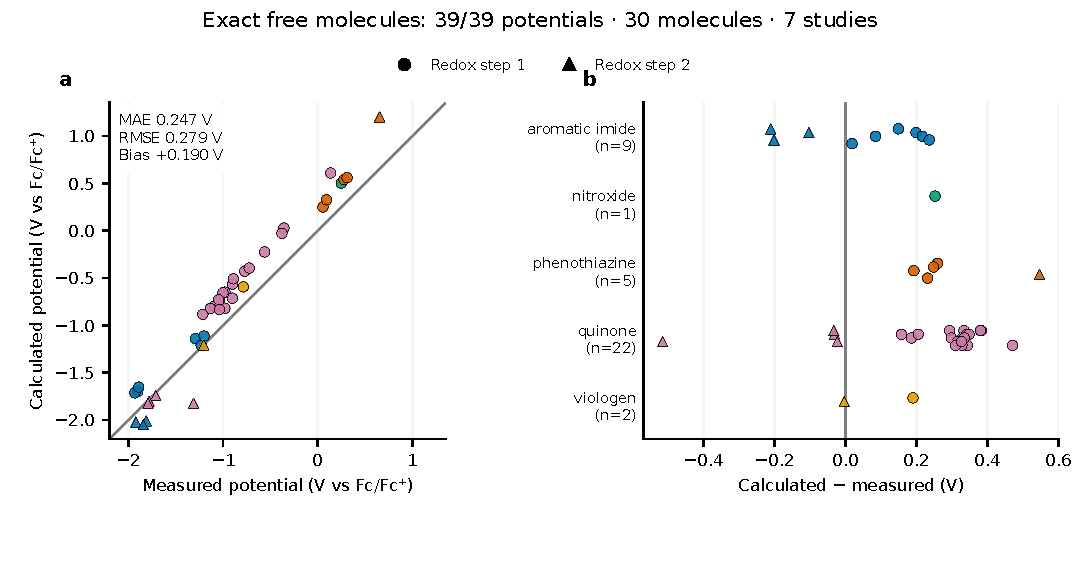
\includegraphics[width=\linewidth]{figures/benchmark.pdf}
\caption{Unfitted comparison of 39 sourced soluble-parent potentials in MeCN. All endpoints are retained. Family and redox-step labels expose uneven coverage and distinguish first- from second-step errors. Bootstrap intervals describe this retrospective panel rather than prospective errors for exact polymer grafts.}
\label{fig:benchmark}\end{figure}

Table~\ref{tab:matchedparents} presents the parent comparisons most closely related to the graft examples. TEMPO and N-ethylphenothiazine first oxidations are too positive by 0.253 and 0.259 V. For benzyl--methyl viologen, the first-reduction error is $+0.190$ V, whereas the second is $-0.003$ V. These are measurements and calculations for matched soluble-parent identities. They are already included in the 39-endpoint panel and supply no additional independent test.
\begin{table}[htbp]\centering\small
\caption{Selected matched parent comparisons from the fixed benchmark. Potentials and signed errors ($E_{\rm calc}-E_{\rm exp}$) are V versus Fc in MeCN. Each source defines its own electrolyte and experimental uncertainty. These parent measurements are distinct from the capped graft models.}
\label{tab:matchedparents}
\begin{tabular}{p{.43\linewidth}rrr}\toprule
Parent and event & Experiment & Calculation & Error\\\midrule
TEMPO, first oxidation\cite{gerken2015tempo} & $+0.249$ & $+0.502$ & $+0.253$\\
N-Ethylphenothiazine, first oxidation\cite{attanayake2019} & $+0.278$ & $+0.537$ & $+0.259$\\
Benzyl--methyl viologen, first reduction\cite{kim2022} & $-0.785$ & $-0.595$ & $+0.190$\\
Benzyl--methyl viologen, second reduction\cite{kim2022} & $-1.204$ & $-1.207$ & $-0.003$\\\bottomrule
\end{tabular}\end{table}

Across the full panel, all 30 first-step errors are positive, with mean $+0.266$ V, while the nine second-step errors have mean $-0.064$ V. All nine paired step spacings are also overestimated in magnitude. Subtracting two potentials calculated against the same Fc couple cancels its contribution exactly. A common reference shift therefore cannot correct the spacing errors, even if it improves a mean potential offset. The near agreement of an individual second step can reflect cancellation of errors.

The computed Fc absolute potential is 4.379 V. Recent solution photoemission work reports a ferrocene adiabatic ionisation energy of $4.94\pm0.05$ eV in MeCN.\cite{baikie2026fc} Our computed reference is a composite solution Gibbs free-energy difference, whereas the cited measurement is an adiabatic ionisation energy. We have not established a matched thermodynamic conversion between them. The comparison motivates investigation of the reference conventions, but does not supply a calibrated error or justify replacing one term of the DFT cycle with the measured value. The opposite first-/second-step residual patterns and the Fc-independent spacing errors require charge-state and solvation contributions to be considered as well. The SI separates this scale comparison from fixed-geometry reference-functional controls.

Post hoc molecule-held-out offsets reduce MAE to 0.158 V with one constant and 0.106 V with separate step constants; the corresponding study-held-out values are 0.182 and 0.124 V. These diagnostics confirm systematic patterns in the residuals within this panel. We do not use them to correct predictions for new grafts. Five neutral-partner diffuse-basis controls shift first potentials by 11.7--35.1 mV, and changing the rotor cutoff gives a largest endpoint span of 25.4 mV. Those limited sensitivities are smaller than the observed molecular error but do not identify its unique cause.\cite{elhajj2024}

\subsection{Viologen connects a demonstrated attachment class to an exact local model}
The viologen example is motivated by a nonaqueous redox-matched battery in which methyl-bipyridinium groups were attached to preformed Merrifield beads.\cite{kim2022} The source reports precursor preparation, grafting in refluxing MeCN and subsequent counterion exchange. Our capped product, registered as \path{search_viologen_b7a4dca7a5e1}, retains the specified local bond but replaces the rest of the polymer by the 4-methylbenzyl model. The experimental soluble benzyl--methyl mediator in Table~\ref{tab:matchedparents} and this capped product are therefore different structures.

The computed graft reductions are $\MolecularFirstReduction$ and $\MolecularSecondReduction$ V versus the matched Fc couple. The states are a dicationic singlet, radical-cation doublet and neutral singlet. The calculated spacing between the reductions is $\MolecularSpacing$ V. These values describe the exact capped model. The demonstrated attachment class provides a practical reason to study this model. The parent errors in Table~\ref{tab:matchedparents}, however, show why its absolute potentials require experimental testing.

The local quaternization in Eq.~\ref{eq:quaternization} gives $\Delta G=\ViologenGraftDG$ \kj\ at the primary cutoff. The three precursor starts span $\ViologenGraftSeedSpan$ \kj, and rotor settings give $\ViologenGraftRotorLow$ to $\ViologenGraftRotorHigh$ \kj. This favorable value refers to separated ions at 298.15 K. The source synthesis uses reflux, and the calculation supplies neither an activation barrier nor a conversion or yield prediction.

Seven optimized chloride-contact outcomes give 1-M association free energies of $\ChlorideAssocMin$ to $\ChlorideAssocMax$ \kj. Duplicate analysis places these outcomes in five numerical groups without assigning statistical weights. The tested contacts are unfavorable under this finite association model. The analysis does not fully account for the dication's counterions, iodide exchange, concentration dependence or salt speciation. These tests examine one assumption of the local reaction model; they do not validate its absolute free energy.

\subsection{Balanced differences separate polymer attachment from neighboring-site response}
Equations~\ref{eq:polylocal} and \ref{eq:nonadditivity} compare different physical effects. PMDI supplies a primary-model illustration: attaching at two sites of a five-repeat chain incurs polymer-minus-local penalties of $+5.34$ and $+6.11$ \kj\ at the primary cutoff, whereas its neighboring-graft response is $-1.86$ \kj. A positive first-site penalty and a negative neighboring-site response can therefore occur in the same finite model. All six site/cutoff penalties are positive, but the small preference between sites changes sign. Full component tables and figures are in the SI. Each graph contributes one minimum, and the exact PMDI installation route remains incompletely established.\cite{bochis1983,hamilton1998}

For viologen, four matched ionic oligomer cycles test adjacent and one-spacer grafts in all-same and alternating backbone configurations (Figure~\ref{fig:occupancy} and Table~\ref{tab:ioniccycles}). The method is the separate r$^2$SCAN-D4/SVP smooth-surface MeCN model, and each component contributes one retained minimum. The neighboring-graft response changes sign at both spacings when the backbone configuration changes. These results illustrate configuration sensitivity within the sampled structures; they do not establish an equilibrium spacing preference. The models have total charge $+4$ when doubly grafted and contain no explicit counterions. The molecular chloride-contact calculations above do not complete a counterion test of these oligomer cycles.
\begin{figure}[htbp]\centering
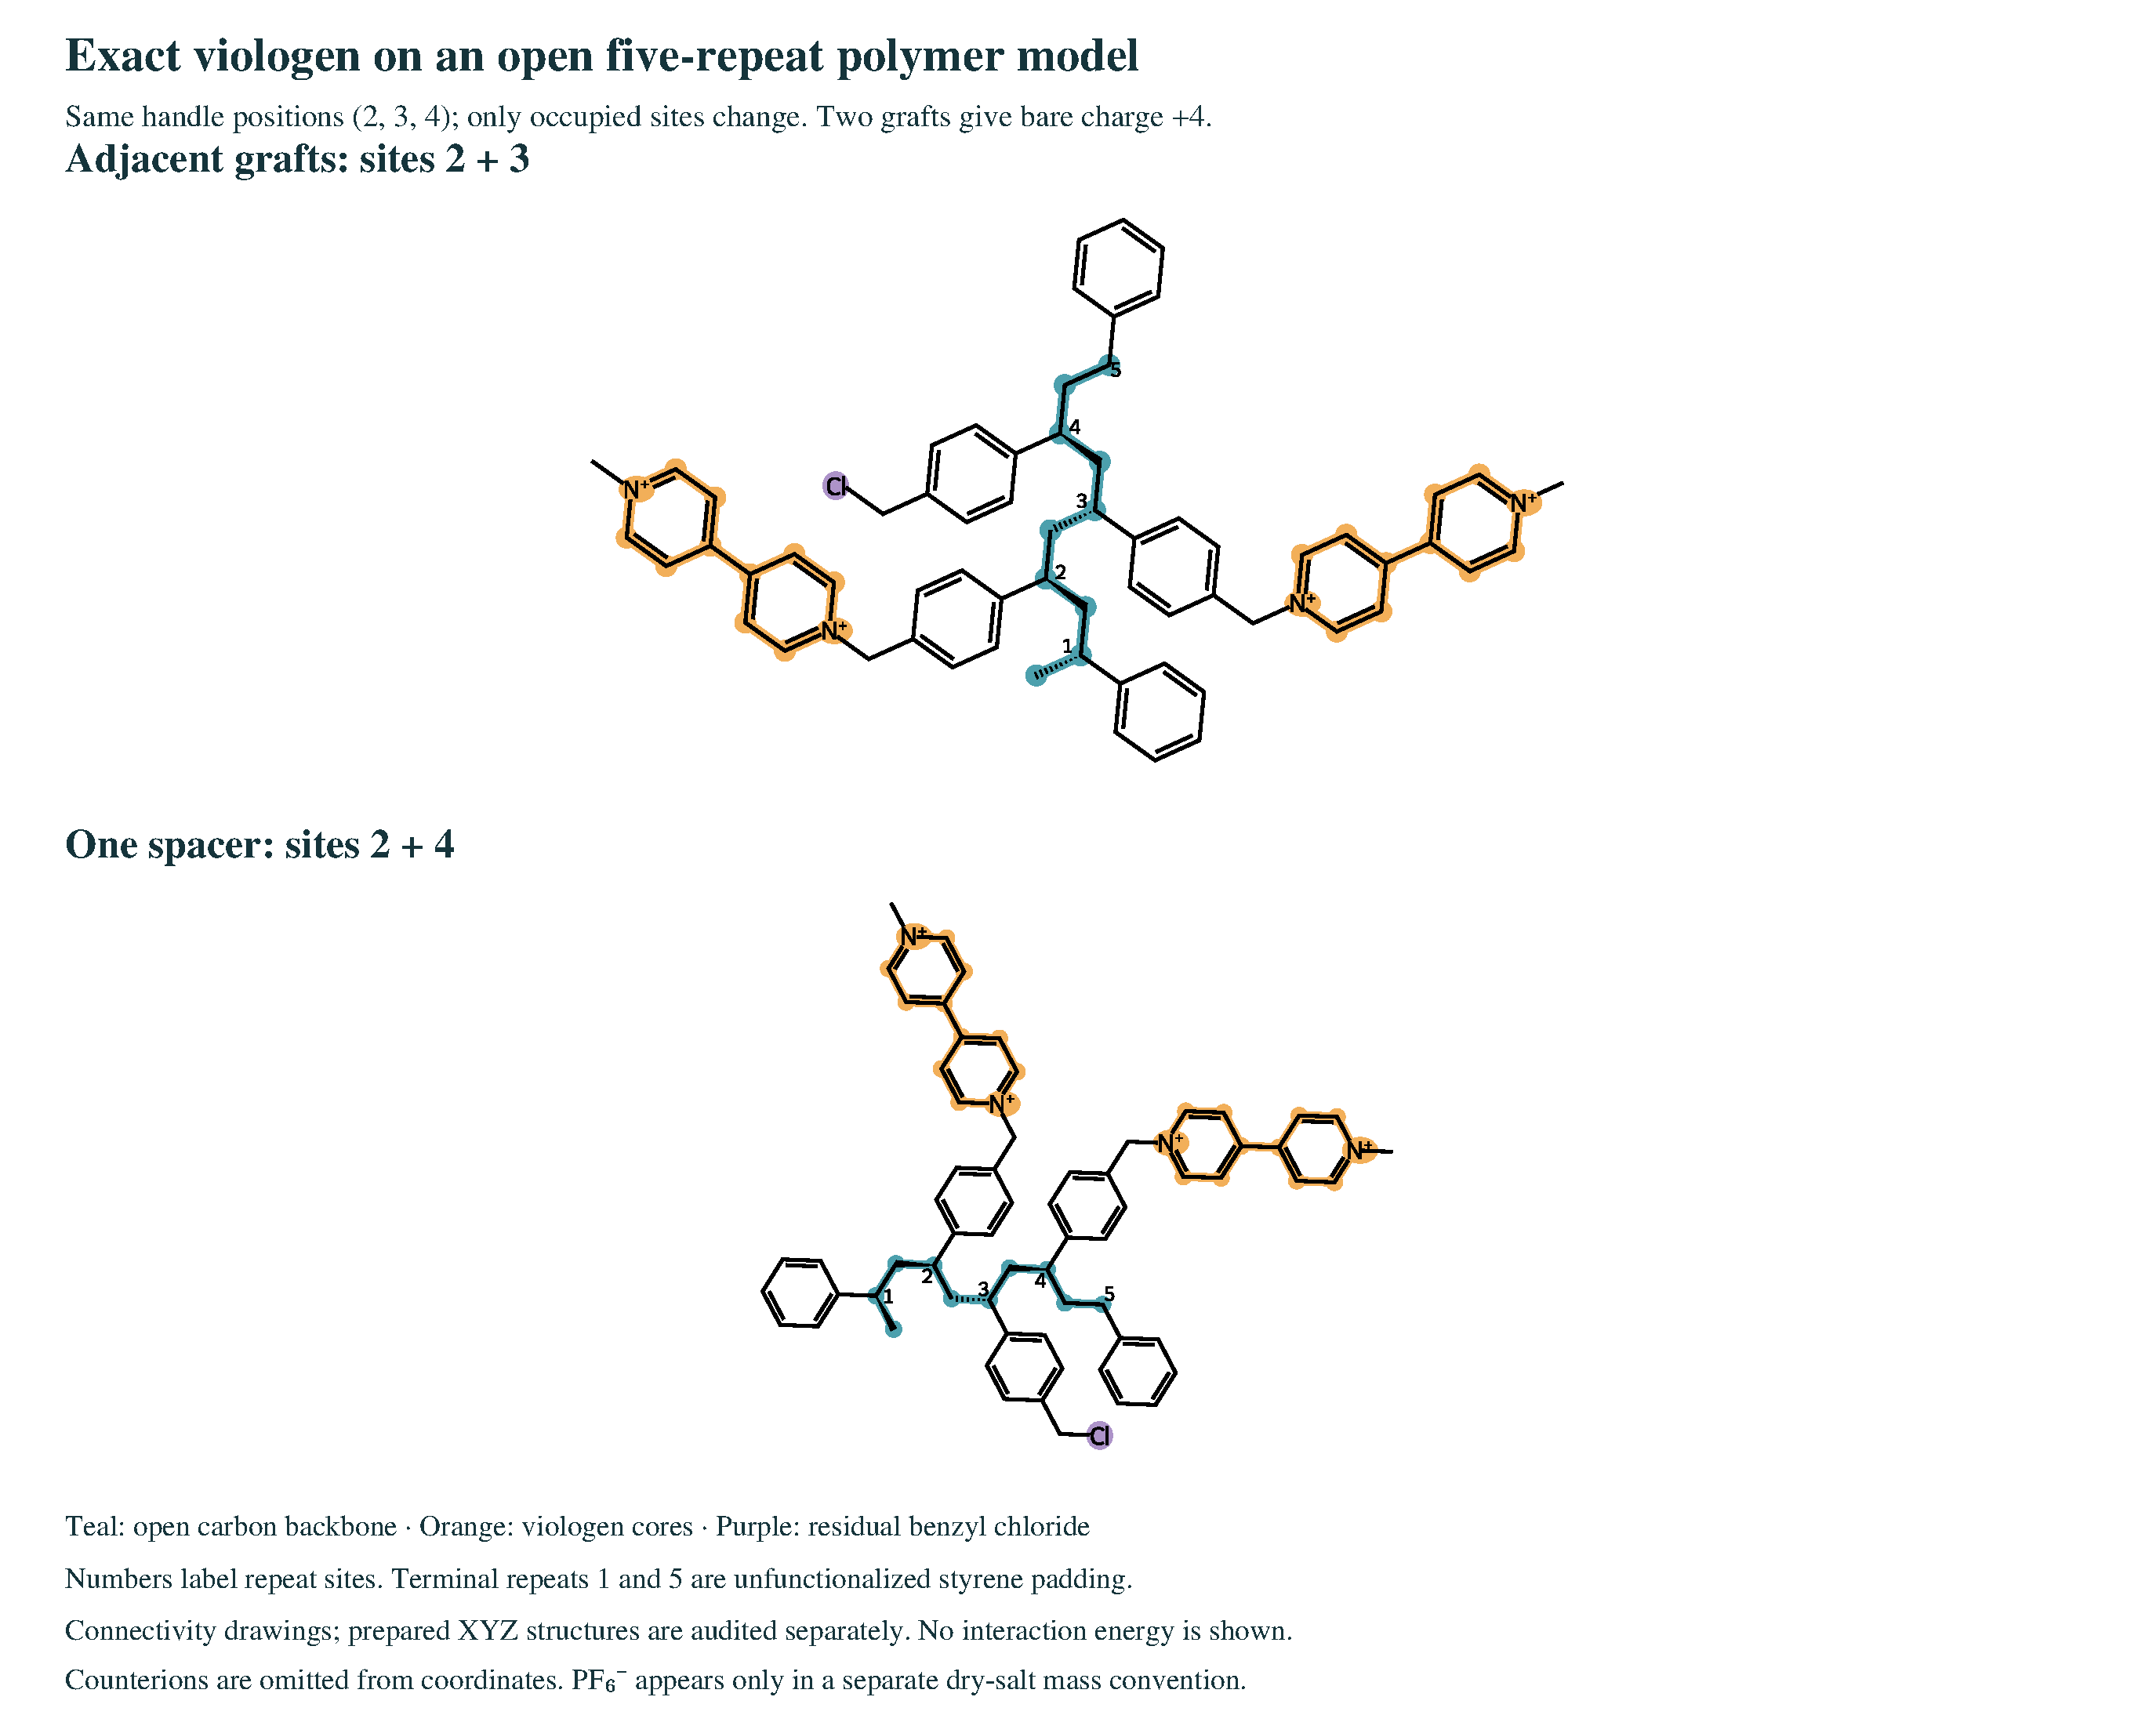
\includegraphics[width=.82\linewidth,height=.68\textheight,keepaspectratio]{figures/viologen_occupancy_construction.pdf}
\caption{Connectivity of the adjacent and one-spacer viologen occupancy models. The open backbone contains five repeats: 1 and 5 are unfunctionalized styrene padding, while the unoccupied reactive site retains benzyl chloride. The drawings define graft positions and the drawn backbone configuration; both configurations in Table~\ref{tab:ioniccycles} have the same site identities. Graph spacing does not prescribe spatial separation. Doubly grafted models have bare charge $+4$ and omit counterions.}
\label{fig:occupancy}\end{figure}

\begin{table}[htbp]\centering\small
\caption{Illustrative ionic viologen neighboring-graft responses, $\Delta\Delta G$ in \kj. Each entry is a balanced four-graph cycle with one retained minimum per graph. The primary cutoff is 50 cm$^{-1}$; the ranges span the tested 25/50/100 cm$^{-1}$ settings and are not uncertainty intervals.}
\label{tab:ioniccycles}
\begin{tabular}{llrr}\toprule
Backbone & Graft spacing & Primary & Cutoff range\\\midrule
All-same & Adjacent & $\IonicAdjacentG$ & $\IonicAdjacentGLow$ to $\IonicAdjacentGHigh$\\
All-same & One spacer & $\IonicSpacerG$ & $\IonicSpacerGLow$ to $\IonicSpacerGHigh$\\
Alternating & Adjacent & $\IonicAlternatingAdjacentG$ & $\IonicAlternatingAdjacentGLow$ to $\IonicAlternatingAdjacentGHigh$\\
Alternating & One spacer & $\IonicAlternatingSpacerG$ & $\IonicAlternatingSpacerGLow$ to $\IonicAlternatingSpacerGHigh$\\\bottomrule
\end{tabular}\end{table}

A separate sampling test illustrates why the conclusions are restricted to retained structures. In the separate occupied-phthalimide control, increasing the number of starts from ten to twenty lowers the finite-set free energy by $\SamplingFiftyAbs$ \kj\ at the primary cutoff, exceeding its $\SamplingTolerance$ \kj\ tolerance. The twenty inputs yield twenty numerical minima. The diagnostic fails across the tested duplicate and rotor settings, and eleven other groups in the cohort remain incomplete. This control does not measure the error of the viologen cycles. It shows why successful minimum checks and rotor-sensitivity tests alone cannot establish convergence of an occupied ensemble. The geometric spacing control also finds close-contact poses for both adjacent and one-spacer graphs, so sequence separation does not by itself exclude spatial contact (SI).

\subsection{Whole-chain nonadditivity differs from direct motif interaction}
The ionic viologen frames allow a second comparison at matched electronic settings (Figure~\ref{fig:ionic-definitions}). Frozen methyl-capped pairs are repulsive in all four MeCN frames, with electronic interactions of $+\MotifMinimumE$ to $+\MotifMaximumE$ \kj. Yet two of the same parent frames have favorable whole-chain electronic nonadditivity. For the adjacent all-same frame, the chain value is $\IonicAdjacentE$ \kj\ and the capped motif interaction is $+\MotifAdjacentE$ \kj. Thus a favorable whole-chain cycle does not, by itself, demonstrate attractive local motifs in this cap model.

The distinction follows from what each quantity compares. The whole-chain cycle contains four separately optimized occupancy graphs. The fragment interaction retains one parent's motif coordinates, removes the aryl linker and backbone and introduces methyl caps. The opposite signs therefore refer to quantities with different definitions. The difference is not a unique decomposition into backbone, deformation and solvent contributions. The tested cap-length span is below $\MotifCapSpan$ \kj, while chemical-cap choice, basis convergence and counterpoise sensitivity remain untested. Both comparisons use electronic energies at matched model settings; neither combines molecular composite $G$ with oligomer $E$.
\begin{figure}[htbp]\centering
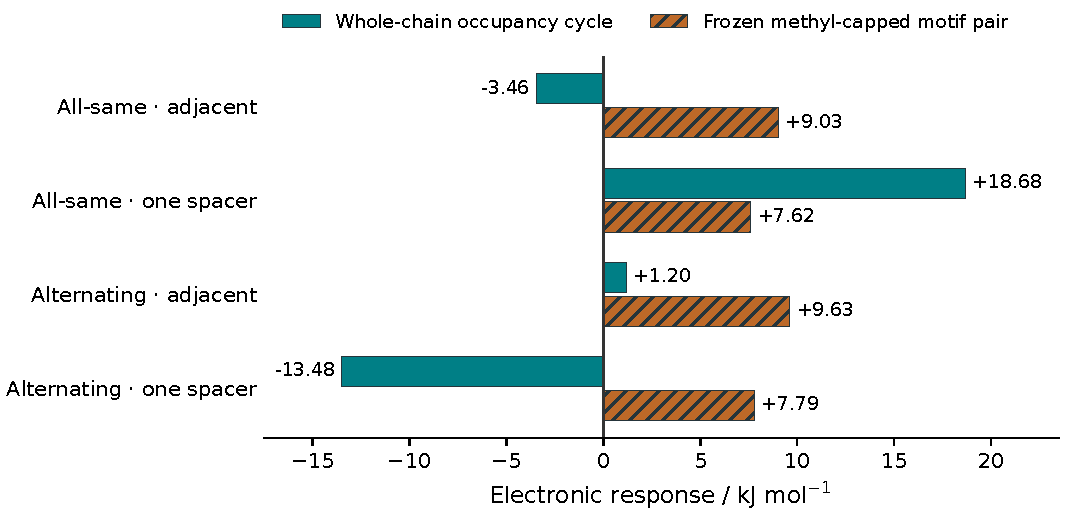
\includegraphics[width=\linewidth]{figures/viologen_interaction_definitions_final.pdf}
\caption{Whole-chain and local electronic responses for four retained ionic viologen frames. The chain cycle is $E(P_{ij})+E(P_0)-E(P_i)-E(P_j)$; the local quantity is $E_{AB}-E_A-E_B$ for frozen methyl-capped motifs. Both use r$^2$SCAN-D4/SVP with the same smooth-surface MeCN model. The opposite signs in two frames concern different quantities and do not define a unique backbone contribution, an association free energy or an electronic coupling.}
\label{fig:ionic-definitions}\end{figure}

\subsection{Implications for selecting grafted redox groups}
The comparisons suggest a practical assessment sequence. Molecular redox predictions should first be tested on matched experimental identities and the relevant redox steps. An installed group should then be specified by its precursor, attachment bond and demonstrated or proposed conditions. Polymer comparisons should use balanced states and report first-site, neighboring-site and local-interaction quantities separately. This sequence connects each molecular descriptor to the chemical question it addresses.

The supporting examples illustrate how other descriptors also depend on their definitions. The exact O-linked TEMPO graft, whose attachment class has NaH/DMF or THF precedent, has a computed oxidation potential of $+0.579$ V versus Fc.\cite{sommerlade2002tempo} Its directional solution-relaxation costs are $\TempoReduction$ and $\TempoOxidation$ eV, differing by $\TempoAsymmetryPercent$\%; this exceeds the declared 5\% diagnostic for a symmetric approximation. These quantities describe directional relaxation costs, not transfer rates. For PMDI, a nominal two-electron molecular capacity of 153.9 mAh g$^{-1}$ becomes a dry-fragment ceiling of 61.2, 98.9 or 124.5 mAh g$^{-1}$ for the specified one-, two- or three-graft models. These composition bounds include scaffold and residual chloride mass but omit unspecified crosslinker, electrolyte and charging counterions. Neither example establishes experimental accessibility or a graft-loading distribution.

Reaction bookkeeping has a similarly specific role. Adding a common base-capture term shifts compatible substitution reactions by the same amount. Their order is therefore unchanged by construction. External acid/base controls reveal a DBU/HCl capture discrepancy of 22.81 \kj, so favorable base-assisted sums cannot be used alone as evidence that a graft will form. The complete reaction panel and its source qualifications are reported in the SI. A demonstrated attachment class and thermodynamic calculations provide complementary evidence; kinetics, selectivity and polymer accessibility remain distinct questions.

The principal limits are molecular prediction error, restricted chemical coverage, incomplete ion speciation and unconverged occupied-polymer sampling. The finite oligomer responses use a different method from the molecular benchmark and do not establish a material ranking, coupling or transport rate. Operating potential windows, accessible electron counts, graft conversion, swelling and cycling stability must be specified and measured for an application. In a redox-matched flow battery, mediator exchange and access to tethered sites are especially relevant.\cite{kim2022} Polymer hopping and backbone-dependent transport provide further reasons to avoid equating an isolated pair interaction with device performance.\cite{hopping2013,oyaizu2008,mohanty2026backbone} The maintained design inventory records structures and available evidence. An incomplete assessment does not demonstrate that every candidate has failed.

\section{Conclusions}
The molecular benchmark identifies a systematic redox-step error: all nine paired step spacings are overestimated, and a common Fc shift cancels from those differences. Explicit matched-parent comparisons also expose first-step errors of approximately 0.19--0.26 V for viologen, TEMPO and phenothiazine examples. These observations identify a specific accuracy problem for molecular screening and motivate validation across the charge states used in a proposed application.

Following an exact viologen graft through its local reaction and oligomer models shows how balanced comparisons add information beyond a molecular potential. Polymer-minus-local attachment, neighboring-graft nonadditivity and frozen motif interaction answer different questions. In the retained ionic frames, favorable whole-chain electronic nonadditivity coexists with repulsive capped motifs, demonstrating why chain-level energetics alone cannot establish local attraction. The present oligomer results are finite-model illustrations whose equilibrium interpretation requires further sampling and ion treatment. Together, the benchmark and matched cycles provide a reproducible basis for evaluating proposed polymer grafts while preserving the distinction between a computed descriptor and a synthesis or material-performance decision.

\section*{Supporting Information}
Experimental benchmark sources, individual endpoints, reference handling and post hoc diagnostics; basis and rotor sensitivity; exact design and route inventory; local reaction components and base-capture controls; PMDI attachment and occupancy comparisons; phthalimide geometry and sampling controls; TEMPO directional relaxation; ionic viologen states and frozen fragments; numerical implementation, restart and portable replay details (PDF). Exact structures and parent-benchmark endpoints are also supplied as CSV, with model context and source records in JSON/TXT.

\section*{Data and Software Availability}
The \href{https://github.com/Ray16/RTFB-materials-research}{project repository} contains development code. A \href{https://github.com/Ray16/RTFB-materials-research/tree/8ee3f78319de744af5cfd022730368a70b4518d6}{commit-pinned source snapshot} preserves the code and evidence context used for this revision. Its \href{https://github.com/Ray16/RTFB-materials-research/tree/8ee3f78319de744af5cfd022730368a70b4518d6/examples/exact_viologen_corrected_replay}{corrected-primary CPU example} reconstructs the molecular redox and local quaternization cycles from ten cached states using NumPy, including nine Hessians and saved-gradient panels. The SI describes raw-state inventories, environments and additional replays. A tagged public release, full raw-data archival deposition and a permanent deposition identifier remain outstanding.

\section*{Author Information}
Authorship, affiliations, corresponding-author details, contributions, funding and competing-interest statements require confirmation by the authors.

\section*{Acknowledgments}
AI tools, including OpenAI Codex and Claude Code, were used during the project to assist with code development, analysis, literature retrieval and manuscript preparation. Computational statements are supported by the recorded calculations and checks described in the Methods and SI. The authors are responsible for reviewing the scientific content, references and this disclosure before submission.

\bibliographystyle{unsrtnat}\bibliography{references,novelty_references}
\clearpage\thispagestyle{empty}
\begin{center}\textbf{For Table of Contents Only}\\[1.5em]
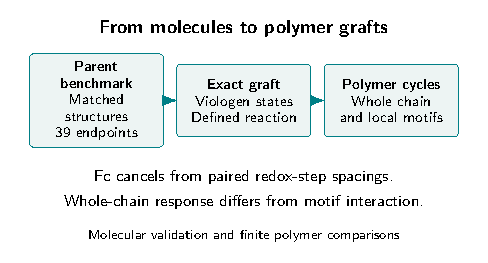
\includegraphics[width=3.25in,height=1.75in]{figures/graphical_abstract.pdf}
\end{center}
\end{document}
